\section{Theoretical Background}
\label{sec:theoretical_background}

\subsection{Machine Learning}
\subsubsection{Types of Machine Learning}
\subsubsection{Classification}

\subsection{Building Blocks of Neural Networks}

\subsubsection{Fully Connected Layer}
\subsubsection{Convolutional Layers}
\subsubsection{Pooling Layers}
\subsubsection{Batch Normalization Layers?}
\subsubsection{Softmax Loss Function}

\subsection{Recurrent Neural Networks}
\subsubsection{Long Short Term Memory Networks}

\subsection{Hybrid Networks}
\label{sec:hybrid_networks}

	\begin{figure}[]
  		\centering
    	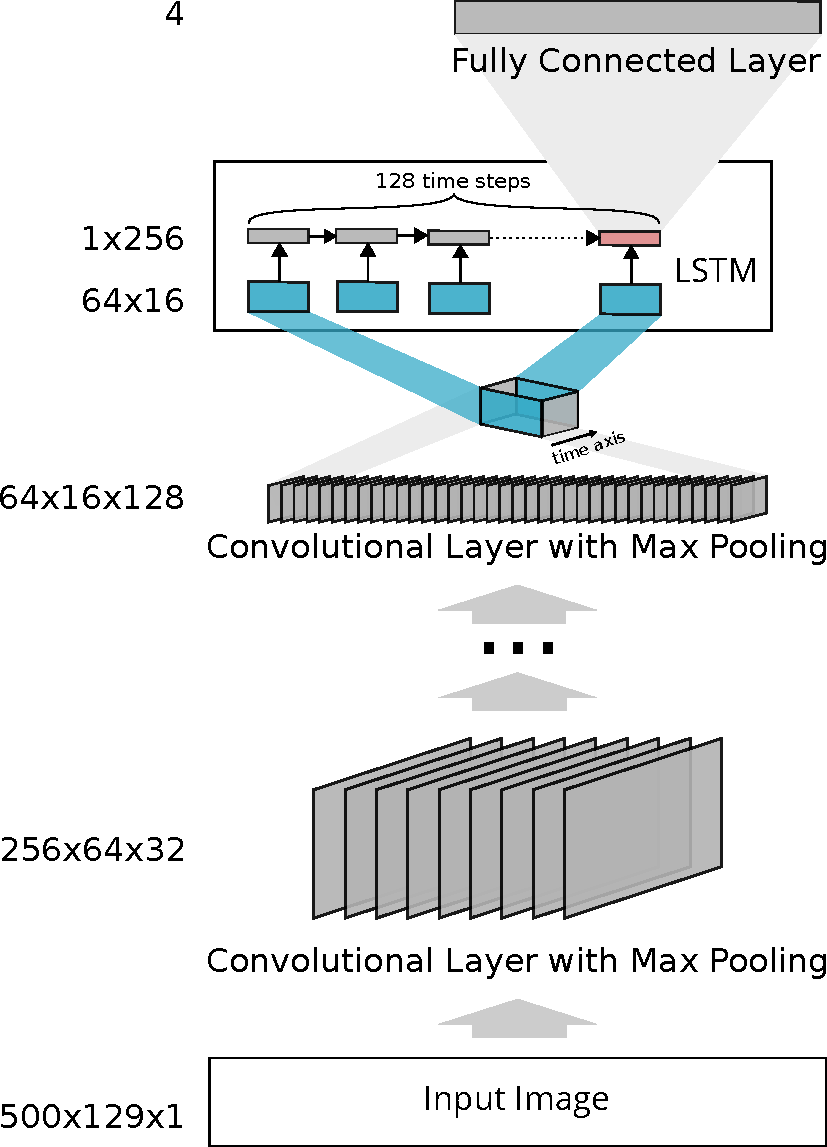
\includegraphics[width=\textwidth, keepaspectratio]{img/crnn.png}
    	\caption{}
    	\label{fig:crnn}
	\end{figure}

    \begin{itemize}
        \item Convolutional Recurrent Neural Networks
    \end{itemize}

\subsection{Audio Representations}
\label{sec:audio_representations}
    \begin{itemize}
        \item MFCC
        \item Spectrogram
        \item Waveform
        \item Mel-scale
        \item frequency --> phoneme --> word --> sentence --> language
    \end{itemize}